\documentclass[fleqn]{article}
\title{Collapsing Heterogeneous Towers of Interpreters}
\author{Michael Buch}
\date{\today}

\usepackage[inline]{enumitem} % inline numbered lists
\usepackage[left=2cm,right=2cm]{geometry}
\usepackage{verbatim} % for comments
\usepackage{graphicx}
\usepackage{amsmath}
\usepackage{amssymb}
\usepackage{amsthm}
\usepackage{textcomp}
\usepackage{txfonts}
%\usepackage{tikz}
%\usetikzlibrary{matrix}
\usepackage{booktabs}
\usepackage{makecell} % For table formatting
\usepackage{multirow} % For table formatting
\renewcommand\theadfont{\bfseries}

\theoremstyle{definition}
\newtheorem{definition}{Definition}[section]
\newcommand{\ts}{\textquotesingle}

\newcommand{\mslang}{$\lambda_{\uparrow\downarrow}$}
\newcommand{\mslangStar}{$\lambda_{\uparrow\downarrow}^*$}
\newcommand{\mevl}{$M_{e}$}

\usepackage{stmaryrd}
\usepackage{hyperref}
\hypersetup{
    colorlinks=true,
    linkcolor=blue,
    filecolor=magenta,
    urlcolor=cyan,
}
\urlstyle{same}

% Code style:
\usepackage{minted}
\RecustomVerbatimEnvironment{Verbatim}{BVerbatim}{}
\renewcommand{\figurename}{Listing}
\usemintedstyle{vs}

\begin{document}
\maketitle
\frenchspacing
\tableofcontents

\begin{abstract}
Intuitively towers of interpreters are a program architecture by which sequences of interpreters interpret each other and a user program is evaluated at the end of this chain. While one can imagine such
construct in everyday applications, prior research made use of towers of interpreters as a foundation to model reflection. As such, towers of interpreters in literature are synonymous with reflective towers and provide a tractable method with which to reason about reflection and design reflective languages. As a result, the assumptions and constraints that govern tower models make them unapplicable to practical or non-functional
settings. Prior formalizations of reflective towers have identified partial evaluation and reflection to harmonize in the development of such towers. We lift several restrictions of reflective towers including reflectivity, meta-circularity and homogeneity of data representation and then construct non-reflective towers
of interpreters to explore how partial evaluation techniques can be used to effectively remove levels of interpretation within such systems. %We then extend formalisms to such setting and go on to generalize previous techniques on partially evaluating towers of interpreters.
\end{abstract}

\section{An Introduction to Towers of Interpreters}
\subsection{What are Interpreters?}
Interpreters vs. compilers
Lines are getting blurry: JIT compilation or more recently Graal
But they Futamura showed they are fundamentally related in an elegant way by three projections that follow from the SMN theorem in recursive function theory
What follows is the study of partial evaluation which lies at the heart of our methodology of collapsing towers of interpreters and is described in more detail in SECTION

\subsection{Reflective Towers}
The earliest mentions of towers of interpreters appeared in the study of reflection in LISP and its derivatives.

\subsubsection{3-LISP, Meta-circularity and Reflection}
In his proposal for a language extension to Lisp called 3-LISP \cite{smith1984reflection}, Smith introduces the notion of a reflective system, a system that is able to reason about itself. The treatment of programs as data is a core concept in the Lisp family of languages and enables  convenient implementations of Lisp interpreters written in Lisp themselves. These are known as \textit{meta-circular} interpreters. Smith argued that there is a distinction between reflection and the ability to reference programs as just ordinary values. Reflection requires a way with which an embedded language can access the structures and state of the process that the embedding lives in. Crucial is the idea of implicit as opposed to explicit information that an evaluator exposes. Smith's idea of reflection is the capability to explicitly instantiate a language construct that was implicit prior. While environment and continuations, which form the state of a tradidional Lisp process, are implicitly passed around, a 3-LISP program can access both these structures explicitly at any point in time. 3-LISP achieves this by way of a, conceptually infinite, \textit{reflective tower}. Smith divides a process into two parts: a \textit{structural field} that consists of a program with accompanying data structures and an evaluator that acts on the structural field. Replacing the evaluator with a meta-circular one then provides a way to construct an infinite reflective tower. In Smith's original model, meta-circular interpreters each with its own environment and structural field, included a builtin \textit{reflective procedure}, which when called provided access to the state, i.e. environment, of it's interpreter. A meta-interpreter, also referred to as ``the ultimate machine'' is the upper-most interpreter in a tower and is itself not evaluated but simply a necessesity for the tower to exist in the first place. Questions of performance, potential uses and a complete model separate from implementation details was provided in subsequent work.
\subsubsection{A Formal Account}
\begin{figure}[t]
	\centering
	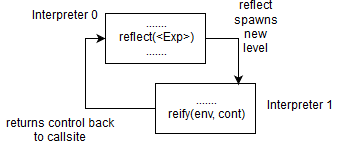
\includegraphics{refl_reif_tower.png}
	\caption{Demonstration of reflection and reification in a two-level tower.}\label{refl_reif_tower}
\end{figure}

Friedman et al. took Smith's account of reflection and decomposed it into distinct operations: \textit{reification} and reflection \cite{friedman1984reification, wand1988mystery}. The authors provide one of the early denotational descriptions of reflective towers assuming a model where an interpreter is a \textit{valuation function} ($\mathcal{E}$) that maps an expression ($Exp$), environment ($E$) and continuation ($K$) to a domain of answers ($A$) and the input values to the interpreter bind to $\epsilon$, $\rho$, $\kappa$ respectively:

\begin{equation}\label{non_refl_eqn}
\mathcal{E}: Exp \rightarrow Env \rightarrow K \rightarrow A = \lambda\epsilon\rho\kappa....
\end{equation}

An open question was how Smith's meta-interpreter \cite{smith1982reflection} could be described in a cohesive framework that relates different levels within a tower through formal semantics. The need for a formalization of reflection was also that earlier work described reflection in terms of reflective towers but which themselves were explained through the use of reflection. To part from such circular reasoning, Friedman et al. defined levels within a tower and their mutual interaction through operators on the state of the valuation function in equation \ref{non_refl_eqn} \cite{friedman1984reification}. Reflection operators take values for expression, environment and continuation and re-install them into the interpreter state. Reification operators provide access to the interpreter state and pass it to the program as values. A packaged up state of $\epsilon$, $\rho$, and $\kappa$ that can be treated as regular values is said to be \textit{reified}. In the context of multiple-levels of interpretation in a tower, calling a reflection operator spawns a new level in the tower with the interpreter state being the one at the time of application. Once evaluation was performed in the new level control is passed back to the interpreter that spawned it. Reification operators package up the state of the interpreter at the level of application and pass it to the expression to be evaluated. Diagramatically this process is shown in figure \ref{refl_reif_tower}.

% Sturdy calls the above a flat tower model

A subsequent study due to Danvy et al. \cite{danvy1988intensions} provides a systematic approach to constructing reflective towers. The authors provide a denotational semantic account of their reflection model similar to the technique described above and realize these formalizations into a language built with a reflective tower called ``Blond''. The authors start with a non-reflective tower and non-meta-circular tower. An assumption that the authors carry throughout their paper is that of single-threadedness. This is both to reduce the complexity of designing an implementation and prevents racey side-effects between concurrent towers. The restriction is that the effects of each level in a tower is the interpretation of the level below it. Any non-interpretative work is performed at the last level of the tower, also referred to as its \textit{edge}. Danvy et al.'s key insight was the need for an intensional description of an interpretative tower that relates the interpreter state at different levels of a tower to the reflection and reification operations. To gain a a better intuition for their description, we summarize Danvy et al.'s model of reflection and reification below.

Adding supscripts to the valuation function from equation \ref{non_refl_eqn} and providing domains for components of the interpreter's state, we get:

\begin{gather}
	\rho_n \in Environment_n = Identifier_n \rightarrow DenotableValue_n \label{denot_non_refl_tower} \\
	\kappa_n \in Continuation_n = DenotableValue_n \rightarrow Answer_n \\
	\mathcal{E}_n: Expression_n \times Environment_n \times Continuation_n \rightarrow Answer_n \\
	\mathcal{E}_n \llbracket interpreter_n \rrbracket \rho_n \kappa_n \simeq \mathcal{E}_{n-1} \label{valuation_fn_non_refl}
\end{gather}

A $DenotableValue_n$ is any valid language construct and its representation as defined by the interpreter at level $n$. A consequence of this formulation is the fact that domains between levels are distinct but connected via the valuation function in equation \ref{valuation_fn_non_refl} and formalizes the earlier notion of an interpreter at level $n$ spawning a new evaluator at $n-1$ through some reflective operation. An even more relevant fact is that according to this denotational model, we are free to choose the representation of denotable values in each level. The authors assume for the rest of their study that levels are identical, however, in our work we assume the exact opposite. None of our levels are identical but can be formulated in the same framework given above. An example would be the denotation of an expression $Exp_0 = (1 + 2)$ at level 0 in our hypothetical tower of $n$ levels. At level $n = 1$ this can be represented as $Exp_1 = (+\;1\;2)_1$ or at level $n = 14$ as $Exp_{14} = (01 + 10)_{14}$, i.e. in binary. In our model we not only keep the notion of non-identical levels and non-metacirularity, but also the concept of a store, which the authors purposefully ommitted to keep the description purely functional.

\begin{equation}
	\begin{split}
		\mathcal{E}_n \llbracket ((reify\;(e\;r\;k)\;body)\;E*) \rrbracket \rho_n \kappa_n \\
		= \mathcal{E}_{n+1} \llbracket body \rrbracket (& [\llbracket e \rrbracket \mapsto (map_n \; \hat{exp_{n}} \llbracket E* \rrbracket) \\
		& \llbracket r \rrbracket \mapsto (\hat{env_{n}}  \rho_n) \\
		& \llbracket k \rrbracket \mapsto (\hat{cont_{n}} \kappa_n)]\rho_{n+1}) \kappa_{n+1} \label{reify_lvls_relation}
	\end{split}
\end{equation}

Equation \ref{reify_lvls_relation} describes the effect of a reification operation, here \textit{reify(e r k)} where e, r and k are the variables that are bound to the expression, environment and continuation of the upper level respectively, between a level $n$ and the level above (i.e. its interpreter) $n+1$.

\begin{equation}
	\begin{split}
	\mathcal{E}_n \llbracket (reflect (E\;R\;K)) \rrbracket \rho_n \kappa_n \\
	= \mathcal{E}_n \llbracket E \rrbracket \rho_n & (\lambda\,a.\mathcal{E}_n \llbracket R \rrbracket \rho_n \\
										& (\lambda\,b.\mathcal{E}_n \llbracket K \rrbracket \rho_n \\
										& (\lambda\,c.\mathcal{E}_{n-1} (\check{exp_n}\,a)(\check{env_n}\,b)(\check{cont_n}\,c)))) \label{refl_lvls_relation}
	\end{split}									
\end{equation}

The reflection operation in relation between two levels, $n$ and the interpreter it interprets $n-1$, is shown in equation \ref{refl_lvls_relation}. The domains for individual reflection and reification operations (superscripted with $\hat{}$ and $\check{}$ respectively), are given equation \ref{refl_reify_types}

\begin{equation}
	\begin{split}
		exp^\wedge_n & : DenotableValue_n \rightarrow Expression_{n-1} \cup {error}		\\
		env^\wedge_n & : DenotableValue_n \rightarrow Environment_{n-1} \cup {error}	\\
		cont^\wedge_n & : DenotableValue_n \rightarrow Continuation_{n-1} \cup {error} 	\\
		exp\,\check{}_{n} & : Expression_{n} \rightarrow DenotableValue_{n+1}			\\
		env\,\check{}_{n} & : Environment_{n} \rightarrow DenotableValue_{n+1}			\\
		cont\,\check{}_{n} & : Continuation_{n} \rightarrow DenotableValue_{n+1}		\label{refl_reify_types}
	\end{split}
\end{equation}

An important observation is that in this model, reification and reflection operators are not commutative. As an example reifying a continuation at level $n$, $cont_n$, followed by reflecting the continuation in level $n+1$ does not yield the same domain when called in reversed order: $\check{cont_{n+1}} \circ \hat{cont_n} \neq \hat{cont_n} \circ \check{cont_{n+1}}$. The expression types given by equations \ref{refl_reify_types} let us explain this trivially by substituting the domains into the inequality.

%by rewriting the compositions as:
%
%\begin{multline}
%	\label{rewrite_composition_fst}
%	(Continuation_{n} \rightarrow DenotableValue_{n+1}) \rightarrow (DenotableValue_{n+1} \\
%	\rightarrow Continuation_{n+1-1} \cup {error}) = Continuation_n
%\end{multline}
%
%\begin{multline}
%	\label{rewrite_composition_snd}
%	(DenotableValue_{n+1} \rightarrow Continuation_{n} \cup {error}) \\ 
%	\rightarrow (Continuation_{n} \rightarrow DenotableValue_{n+1}) = DenotableValue_{n+1} \cup{error}
%\end{multline}

A less formal explanation of this statement is in terms of the possible values reflection versus reification can result in. Reflection spawns a new interpreter that can yield any result, including an error. Then reifying an error would not yield a valid interpreter state. If one reflects a reified expression it by definition corresponds to simple evaluation in the current interpreter. The importance of this is that this restricts us from being able to fully explain a reflective tower model and valuation functions that act on a level below, $\mathcal{E}^{-1}_n$. If we are not able to provide a definition for reflection and reification at interpreters below any level $n$ we will not have a full description of a reflective tower. This gives a denotational account for the metacontinuations that 3-LISP originally introduced. It was to deal with exaclty this discrepancy in the compositionality of reflection and reification operations. Danvy et al. then add meta-continuations into the equations previously described and their purpose is to describe the continuation that accepts the result of the interpreter it interprets.

\subsection{Collapsing Towers}
Taking a traditional model of interpretation, a conceptually infinite tower of interpreters adds evaluation overhead solely for the purpose of achieving reflection. In the original proposals of the reflective tower models only minimal attention was given to the imposed cost of performing new interpretation at each level of a tower. BLOND/STURDY both hint at partial evaluation potentially being a tool capable of removing some of this overhead by specializing individual levels to the interpreters below.

\subsubsection{Compiling Reflective Languages}
\cite{asai1996duplication}: Language ``Black''; has early uses of the act of collapsing modes of interpretation in a reflective setting. Its reflective model is closer to 3-LISP than to Blond or Brown
\cite{asai2015compiling}

The Truffle framework due to Wh{\"u}rthinger et al. \cite{wurthinger2017practical} demonstrate a practical partial evluation framework for interpreters independent of language by providing a language and interpreter specifically designed to partially evaluate and thus collect as much information about a dynamic language at run time as possible.

\subsubsection{Examples}
Examples drawn from paper on collapsing towers \cite{amin2017collapsing}:
\begin{itemize}
	\item Regular expression matcher <- Evaluator <- Virtual Machine
	\begin{itemize}
		\item Generate low-level VM code for a matcher specialized to one regex (through arbitrary number of intermediate interpreters)
	\end{itemize}
	\item Modified evaluator <- Evaluator <- Virtual Machine
	\begin{itemize}
		\item Modified for tracing/counting calls/be in CPS
		\item Under modified semantics "interpreters become program transformers". E.g. CPS interpreter becomes CPS transformer
	\end{itemize}
\end{itemize}

Recent work following on from Asai's work has demonstrated the ability to compile an potentially infinite tower of interpreters with dynamically changing semantics of individual levels using novel applications of normalization-by-evaluation \cite{amin2017collapsing}. Our work is motivated by following, rephrased, of question posed in the conclusion of their work: is it possible to extend the framework to practical towers and how?

\subsection{Heterogeneity}
A central part of our study revolves around the notion of heterogeneous towers. Prior work on towers of interpreters that inspired some these concepts includes Sturdy's work on the Platypus language framework that provided a mixed-language interpreter built from a reflective tower \cite{sturdy1993lisp}, Jones et al.'s Mix partial evaluator \cite{jones1989mix} in which systems consisting of multiple levels of interpreters could be partially evaluated and Amin et al.'s study of collapsing towers of interpreters in which the authors present a technique for turning systems of meta-circular interpreters into one-pass compilers. We continue from where the latter left of, namely the question of how one might achieve the effect of compiling multiple interpreters in heterogeneous settings. Our definition of \textit{heterogeneous} is as follows:
\theoremstyle{definition}
\begin{definition}
	Towers of interpreters are systems of interpreters, $I_0, I_1, ..., I_n$ where $n \in \mathbb R_{\ge 0}$ and $I_n$ determines an interpreter at level $n$ interpreted by $I_{n-1}$, written in language $L$ such that $L_{I_n}$ is the language interpreter $I_n$ is written in.
\end{definition}

A level here is analogous to an instance of an interpreter within the tower and as such level $n$ implies $I_n$ if not mentioned explicitly otherwise.

\begin{definition}
	Heterogeneous towers of interpreters are towers which exhibit following properties:
	\begin{enumerate}
		\item For any two levels $n, m \in \mathbb R_{\ge 0}, L_{I_n} \not\equiv L_{I_m}$
		\item For any two levels $n, m \in \mathbb R_{\ge 0}, L_{I_n} \not\blacktriangleleft L_{I_m}$, where $\blacktriangleleft$ implies access to the left-hand side interpreter's state and $m \ge n$
		\item For any language used in the tower $L_m \in \Sigma_L$, $\exists L_a \not\in \Sigma_L.L_m \blacktriangleleft L_c \land L_c \blacktriangleleft L_c$
	\end{enumerate}
\end{definition}\label{def:het}
A common situation where one find such properties within a system of languages is the embedding of domain-specific languages (DLSs) and we describe the consequence of these properties in the subsequent sections.

\subsubsection{Absence of: Meta-circularity}
The first constraint imposed by definition \ref{def:het} is that of necessarily mixed languages between levels of an interpretative tower. A practical challenge this poses for partial evaluators is the inability to reuse language facilities between levels of a tower. This also implies that one cannot define reflection and reification procedures as in 3-LISP \cite{smith1984reflection}, Blond \cite{danvy1988intensions}, Black \cite{asai1996duplication} or Pink \cite{amin2017collapsing}.

\subsubsection{Absence of: Reflectivity}
The ability to introspect and change the state of an interpreter during execution is a tool reflective languages use for implementation of debuggers, tracers or even language features. With reflection, however, programs can begin to become difficult to reason about and the extent of control of potentially destructive operations on a running interpreter's semantics introduces overhead. Reflection in reflective towers implies the ability to modify an interpreter's interpreter. Hierarchies of language embeddings as the ones we are interested in rarely provide reflective capabilities at every part of the embedding.

\subsubsection{Mixed Language Systems}
An early mention of non-reflective and non-metacircular towers was provided in the first step of Danvy's systematic description of the reflective tower model \cite{danvy1988intensions}. However, potential consequences were not further investigated in their study. However, their denotational explanation of general interpretation and description of interpretater state served as a useful foundation for later work and our current study.

An extensive look at mixed languages in reflective towers was performed in chapter 5 of Sturdy's thesis \cite{sturdy1993lisp} where he highlighted the importance of supporting a mixture of languages within a interpretation framework. Multi-layer systems such as YACC and C or Shell and Make are common practice. Sturdy goes on to introduce into his framework support for mixed languages that transform to a Lisp parse tree to fit the reflective tower model. Our work is similar in its commmon representation of languages, however, we remove the requirement of reflectivity and argue that this provides a convenient way of collapsing, through partial evaluation a mixed level tower of interpreters. While Sturdy's framework \textit{Platypus} is a reflective interpretation of mixed languages, we construct a non-reflective tower consisting of mixed languages.

The mix parial evluation framework \cite{jones1989mix}, Jones et al. demonstrate the PE of a simple interpreter into a language called Mixwell developed by the authors. This is similar in spirit to our framework except it is smaller in height. (section 5 of the paper \cite{jones1989mix}). also mentions removal of layers of metainterpretation in its conclusion

Recent work due to Sampson et al. \cite{sampson2017static} differentiates between value splicing and materialization. Materialization and cross-stage references are used to persist information across stages. This provides a possible solution to pass information about staging decisions across levels.

Partial Evaluation of Machine Code

Put together, the three properties imposed by definition \ref{def:het} encourage a generalized solution irregardless of the language or structure of the tower at hand.

One of the earliest serious mentions of collapsing levels of interpretation using partial evaluation was \cite{sturdy1993lisp}

\section{Problems}
To put our work and motivation into context consider following program architecture (originally described in \cite{amin2017collapsing}): some user script is executed by a Python interpreter running on a JavaScript emulator of a x86 CPU, all of which is run within a browser that eventually is executed on hardware. This construction resembles a practical realization of our defintion of heterogeneity in towers of interpreters, or in this case a tower of languages. Although such scenario might seem far-fetched, other forms of towers such as domain-specific languages embedded within a host are a form of tower of interpreters. Our study presents a systematic construction of a tower that resembles the structure of the tower we describe above: each level's language is different from the one it interprets and strict interpretation, where implementation is infeasible, is replaced with compilation. In addition to the issues outlined in previous work specifically on towers of interpreters, we also touch on and evaluate our results against the collection of open challenges described by Jones \cite{jones1988challenging} some of which have been tackled since but some of which remain open questions, such as the extent to which partial evaluators can perform the work by optimizing compilers and code generation by partial evaluators whose target language is different that its source. % paragraphs 3.6 - 4 in cited paper; is 4.2 basically our approach?

What we envision (with reference to this hypothetical setting) is handling the two following cases:
\begin{enumerate}
	\item A one-off run of a python script on top of this stack should be collapsed by bypassing the emulator interpretation
	\item A continuously running emulator evaluating a continuously running python interpreter should collapse individual runs of interpretation while respecting the dynamically changing environment
	\begin{itemize}
		\item Here a dynamically changing environment also implies effects that are capable of changing the semantics of interpreters within the tower at runtime
		\item In literature, the closest to compiling a dynamically changing tower is \cite{asai1997partial, amin2017collapsing} (for a \textit{reflective} language Black) and GraalVM \cite{wurthinger2013one}
	\end{itemize}
\end{enumerate}
To tackle the first of these problems we construct a similar yet condensed form of the setting as shown in \ref{secd_tower_arch}.

\section{Why do we want to collapse towers?}
The main reason is performance. The key realization of partial evaluation that lead to its development is that interpreters do redundant work but we can make it so they don't. Program specialization is simple and attractive on paper but poses significant engineering challenges and has not seen widespread adoption (until recent increasingly successful work on interpreter virtualization \cite{wurthinger2013one}).

Binding time analysis is one of the obstacles of program specialization. The program specializer needs to decide, either automatically or with assistance from the programmer, which data to treat as static and which as dynamic. Simple divisions
can lead to code explosion or inefficient code generation, or worse, to non-termination of the specializer. This problem is known as \textit{division} and is one of the key differences between offline and online PE techniques \cite{jones1993partial}.

An interesting consequence of collapsing towers of interpreters demonstrated in \cite{amin2017collapsing} paper is the ability to derive translators in the process of collapsing.

\begin{figure}[t]
	\centering
	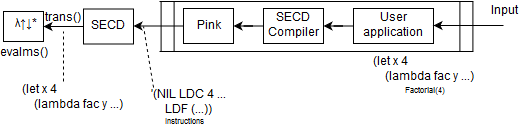
\includegraphics[scale=0.75]{secd_arch.png}
	\caption{``Effectively functional'' \mslangStar with SECD tower above it}\label{secd_tower_arch}
\end{figure}

\subsection{Example of Deriving Translators}
A trivial but useful example is logging. Given the tower in figure \ref{logging_translator_tower} we want to keep the added \textit{useful} behaviour of $I_3$ while removing the \textit{unuseful} other work of interpreting an intermediate representation. The interpretation
of the IR of the level above is a mere accidental consequence of design instead of a necessity. We claim this work to be \textit{interpretative overhead} and defer its quantification by benchmarks to a later section.

Collapsing the tower achieves exactly what we wanted, base-language (here the compilation target language) expressions including logging specialized to the user-level program.

A restriction with this method is its reliance on meta-circularity and reflection and other unsafe techniques:
\begin{itemize}
	\item we are able ``inject'' the logging evaluator into tower because of its meta-circularity
	\item we expose staging operators throughout the tower through simple string manipulation
	\item instrumentation relies on meta-circularity since we simply redefine how constructs are evaluated before injecting the evaluator
	\item modification of semantics of the tower are done via reflection (ELABORATE)
\end{itemize}

\section{Contributions}
% TODO: interpreters should be evaluators
%TODO: stronger first sentence that summarizes contributions, non-metacircular -> heterogeneous
In our study we investigate previous work on collapsing towers of interpreters and aim to take another step towards applying these techniques to real-world settings. We demonstrate that given a multi-level language and a lift operator we can stage individual interpreters in a sequence of non-metacircular interpreters and effectively generate code specialized for a given program eliminating interpretative overhead in the process. As part of the development of this framework our contributions include:
\begin{enumerate*}[label=(\arabic*)]
	\item the development of extensions to the SECD machine that allow it to be staged
	\item implementation of a compiler from a minimal LISP-style language to instructions of the staged SECD machine
	\item demonstration of collapsing towers of interpreters built on top of the aforementioned SECD machine
	\item evaluate the effect of staging at different interpreters within a tower of interpreters
	\item demonstrate the ability to use NbE-style lift operators to perform partial evaluation across levels in the tower that are compilers
	\item and finally evaluation of the structure of the generated code and possible optimizations
\end{enumerate*}.

We deviate from traditional research in reflective towers in that we do not develop a separate language that demonstrates reflective tower capabilities and part from the constraints of metacircularity and reflection.
Instead of generating levels in the tower dynamically through reflection and reification operators we construct a pre-determined tower resembling towers of interpreters in practice. We demonstrate initially how meta-circularity and reflection eases the collapsing process and then wire the tower in a way that breaks key implicit assumptions of said technique. Finally we propose a generalization of the original framework that deals with the constraints such a semantic gaps and lack of reflection and reification. We evaluate the framework on a set of abstract machines that are convenient to implement in Lisp-like fashion but are capable of modelling a broad set of functional and non-functional language properties.

\cite{jones1993partial}: page 26. Only recently has partial evaluation seen growing adoption with frameworks such as Scala's LMS \cite{rompf2010lightweight} or Oracle's GraalVM \cite{wurthinger2013one}. The design space of partial evaluators is multi-faceted and considerations include:
\begin{itemize}
	\item use of mixed languages (Futamura's mix for compilation requires same PE input language as mix is written in)
	\item accept different types of interpreters with different semantics (this is what we partly address) (and what GraalVM addresses?)
	\item performance
	\item BTA strategy: automatic or manual? offline or online? how to deal with non-termination?
	\item Heuristics for guiding PE to produce efficient/desirable code (e.g. you cannot say of a compiler that it doesn't produce more valuable program transformation. But PE's accept that some applications do not warrant it. How to detect such situations?)
\end{itemize}

semantic gap has been discussed previously as a challenge outstanding in the study of partial evaluation.

Chapter 17: specifcies partial evaluation in the context of general program transformation and outlines PE research areas

TODO:
staging vs pe
partial evaluatability of SECD (and other linear interpreters/small step semantics vs denotational/big step/recursive descent parsers)
retaining info in PE of TDPE style (our strategy is thunks)
contribution: was natural to start with EBASE but uncovered problems BLANK
tying the knot in the code instead of data
transfer whiteboard diagram
are able to stage/lift through compiler/translator
structurally similar/equal to javascript tower
implementations:
	1. regular expression matcher (on metaeval or in place of metaeval)
	2. try/catch
	3. using cps adding amb (needs set! and store => turn metaeval into cesk machine (possible because SECD supports recursion, lambdas, letrec, etc.))
Our collapsing strategy is based on the fact that we can choose to either evaluate code or generate code which is an inherent property of the multi-level language base \mslang. Thus in a realistic tower base needs to be a multi-level language

Partial evaluators can be thought of as lightweight optimizing compilers targeting specific optimization goals

Red thread:
reflective towers->formalization of towers (first mention of PE by Sturdy and Blond) and first hint at heterogeneity->shift perspective to how such model is realizable->what is evaluation overhead of such models->compiling towers->polymorphic lift->define heterogeneity->find abstract machine for our purpose->SECD->requires side-effects->tie not in code instead of data->benchmarks+code comparisons+optimizations->extend tower->more benchmarks

% https://tex.stackexchange.com/questions/181366/drawing-tombstone-diagrams
% https://proglang.informatik.uni-freiburg.de/teaching/compilerbau/2004/T-diagrams.pdf
% TODO: use http://mirror.its.dal.ca/ctan/macros/latex/contrib/semantic/semantic.pdf package to draw diagram
% TODO: draw diagram for practical tower as well
\begin{figure}[t]
	\centering
	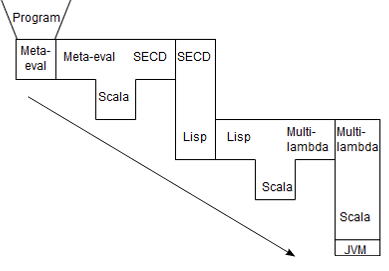
\includegraphics[scale=2]{tombstone_tower.png}
	\label{fig:tombstone}
	\caption{A tombstone digram representation of our framework}
\end{figure}

For the rest of this thesis we systematically describe the process by which we create a heteregeneous tower of interpreters and incrementally collapse it. The aim of the following sections is to enumerate the steps we took to create a tower of interpreters as shown in figure \ref{fig:tombstone} and our experiments on it. Section SECTION describes the original framework due to Amin et al. \cite{amin2017collapsing} which we extend for the purposes of our work. The sections after (SECTIONS 1 2 3), each represent the addition of an individual layer in the tower. We conclude with an evaluation of experimental results followed by a discussion of potential future work.

\section{Background}
\subsection{Type-Directed Partial Evluation (TDPE)}
NbE resources:
Useful \href{http://cs.ioc.ee/ewscs/2009/dybjer/mainPalmse-revised.pdf}{Slides}
\href{http://www.cse.chalmers.se/~abela/univnbe.pdf}{NBE paper}
\href{http://homepages.inf.ed.ac.uk/slindley/nbe/nbe-cambridge2016.pdf}{More slides}
\href{https://www.microsoft.com/en-us/research/wp-content/uploads/2016/07/supercomp-by-eval.pdf?from=http%3A%2F%2Fresearch.microsoft.com%2Fen-us%2Fum%2Fpeople%2Fsimonpj%2Fpapers%2Fsupercompilation%2Fsupercomp-by-eval.pdf}{Supercompilation by Evaluation}
\href{http://citeseerx.ist.psu.edu/viewdoc/download?doi=10.1.1.630.2123&rep=rep1&type=pdf}{Supercompilation and Normalization by Evaluation}

Alternative techniques include syntax directed partial evaluation and off-line partial evaluation
Futamura's second project showed the direct relationship between an interpreter and a compiler -> hard to realize
Jone's et al. developed MIX which was the first self-applicable PE that operated on a language developed by the same authors called MIXWELL.
MIX innovated by making binding-time decisions offline as opposed to during partial evaluation time using source annotations for the PE
However as noted in \cite{grobauer2001second}, traditionally partial evaluation worked on untyped languages where a single universal datatype could represent all static values
PE of typed languages was one of the challenges with PE outlined by Jones \cite{jones1988challenging}.

Differences to traditional syntax-directed offline partial evaluators (like MIX):
* binding time is automatic (or requires annotations only on inputs to program e.g. like in Pink, which requires knowledege of how the binding-time works. TDPE only requires annotations on base types from which product, sum and function types' binding-times can be deduced. Pink does not necessarily have a binding time analysis step which makes it slightly more convenient for manual annotation)
* type-directed means we use the type of a term to guide the normalization (i.e. ``extraction function'' is parameterized by type)
* TDPE reuses underlying evaluator to perform static evaluation vs code generation. Traditionally these are performed by the partial evaluator separately in the form of symbolic computation on the source. Pink takes the former approach

In \cite{danvy1999type} Danvy builts a language in ML that supports and reflection (section 1) and then shows how partial evaluation of can be achieved using a ``normalization function'':
%In  summary,  if  one  implements  the  two-level  lambda-calculus  as  in  Sec-tion  1.3, then reifying  a simply typed,  closed, and completely static  higher-order  function  into  a  dynamic  expression  automatically  yields  a  representation  of  its  normal form.  In the rest  of this section,  we illustrate this phenomenon  with  de-compilation,  before  turning to the  implementation  of  a normalization  function  in  ML.

page 379 explains role of let-insertion
Our framework uses the Eijiro Sumii  approach

page 388: actual description of TDPE
"We  define  type-directed  partial  evaluation  as normalization  by  evaluation  over  ML values"

page 403: benefits of NbE

\cite{jones1993partial} page 103: monovariance, polyvariance, congruence in PE

\subsection{Staging}
There are two types of partial evaluation methodologies \cite{jones1993partial}:
\begin{itemize}
	\item Offline partial evaluation
	\item Online partial evaluation \cite{cook2011tutorial}
\end{itemize}
Namin et al. \cite{amin2017collapsing}, propose two languages Pink and Purple. Pink uses a form of online partial evaluation but requires manual staging facilities. Purple relies on LMS for automatic binding time analysis and staging
which limits it to offline partial evaluation and thus relies on further optimization heuristics to achieve the same level of program specialization in the generated code as Pink.
at its heart it uses the fact that $\beta$-reduction to $\beta$-normal form can be viewed as a form of specialization (taken further by NbE \cite{berger1991inverse,berger1998normalization})
``NbE'' extracts the normal form from its meaning (i.e. semantics -> syntax or in our case Val -> Exp which is done via the ``lift'' operator in \mslang)

Staging and partial-evaluation are closely related but are often misused interchangeably. Staging is used to split an evaluation into multiple phases, or stages. For instance, a traditional compiler model consists of a compilation pipeline where a program is transformed and passed on to another stage. This is one of the reasons we can call a staged interpreter a compiler, since instead of evaluating source in one go the interpretation is split into multiple stages of program transformation.

A widespread technique for implementing partial evaluators is by staging an interpreter but this need not be the case. COUNTER-EXAMPLE

\subsection{Abstract Machines}

\section{Level 1: \mslang}\label{sec:mslang}
\begin{itemize}
	\item Stage polymorphism \cite{ofenbeck2017staging}: ``abstract over staging decisions'' i.e. single program generator can produce code that is specialized in many different ways (instance of the Fourth Futamura Projection? \cite{gluck2009there}) 
	\item Multi-level base evaluator written in \mslang: supports staging operators (\textbf{polymorphic Lift})
	\item Modify other interpreters: make them \textbf{stage polymorphic}, i.e. commands either evaluate code (like an interpreter) or generate code (like a translator)
	\item Stage only user-most interpreter: \textit{wire tower} such that the \textbf{staging commands in $L_{n}$ are interpreted directly in terms of staging commands in $L_{0}$} i.e. staging commands pass through all other layers handing down commands to layers below without performing any staging commands
	\item Non-reflective method: meta-circular evaluator \textbf{Pink} => collapse arbitrary levels of ``self-interpretation''
	\item By abstracting over staging decisions one can write the same program to both perform staging or evaluate directly \cite{amin2017collapsing} (maybe-lift)
	\item \mslang features:
	\begin{itemize}
		\item \textit{run residual code}
		\item binding-time/stage polymorphism \cite{henglein1994polymorphic}
		\item preserves execution order of future-stage expressions
		\item does not require type system or static analysis
		\begin{itemize}
			\item TDPE \cite{danvy1999type} (great explanation also at \cite{grobauer2001second}): \textbf{polymorphic Lift} operator turns static values into dynamic (future-stage) expressions
		\end{itemize}
	\end{itemize}
\end{itemize}

In partial evaluation terms, the configurations, i.e. set of run-time computational states, is stored in stBlock while the division, i.e. denotation of static vs dynamic values 

\subsection{\mslang Overview}
Since our work is based on the multi-level language, \mslang, developed by Amin et al. \cite{amin2017collapsing} we provide a summary of the core language which is a call-by-value $\lambda$-calculus split into two evaluation contexts, one in which expressions are code and the other in which expressions normalize to values. It also features a NbE style lift operator that forms tool by which partial evaluation is achieved. The LISP front-end is described in figure FIGURE. It is a LISP derivative that has support for non-mutable list and cons-cell operations, the lift operator for staging and recursive self-referencing lambdas.

%Our language extends Pink with side effects and a stack machine that makes use of pointer like semantics for Lisp-like cons pairs. Thus we build on top of the NBE-style lift operator for staging. However, calling into
%the base-level lift requires knowledge about its use to be passed from the layers above. We can employ several strategies of doing this:
%\begin{itemize}
%	\item A basic approach exposes the base layer staging operation to the level above. This is how the original Pink implementation works.
%	\item At every layer \textit{deduce} whether we need to call the underlying interpreter staging operator
%	\begin{itemize}
%		\item This requires every level to include an implementation of such staging operations
%	\end{itemize}
%	\item A mixture of passing staging operations to the layer below or implementing ones own operators
%	\item Find a method of passing staging decisions through each layer in a generic way without intrusive changes to the evaluators of the layers
%	\item Decide about calling staging operations at a particular point in the tower and apply previous points
%\end{itemize}
%We are interested in the last two point. In heterogeneous and practical towers a programmer does not have the liberty to introduce intrusive changes along each layer.

The original Pink implementation assumes we are allowed to make arbitrary changes to evaluators. It effectively adds tags to the emitted representation of a layer above and lets the layer below infer from these tags what tag it itself should pass to the next layer, eventually calling the base-level Lift term.

How are stages encoded? dynamic vs. static (e.g. see MetaOcaml or TDPE's ML extensions)

\subsection{Changes to \mslang}
Since SECD is a stack-based virtual machine all operations and data storage is performed on one of the four stack registers. By the principle of \textit{division} in partial evaluators CITE, we want to be able to separate static and dynamic values to prevent undesired behaviour in our partial evaluator (EXAMPLE OF NON-TERMINATION). A minor extension we add to the original framework is the ability to lift nested tuples as opposed to only two-element tuples. This addition to the small-step semantics is shown in FIGURE.

To reduce the amount of generated code we add logic within \mslang's \textit{reflect} that reduces purely static expressions. Reducible expressions include arithmetic and list access operations.

SHOW OPERATIONAL SEMANTICS

% Power of a dedicated "lift" instruction -> turns interpreter into compiler with ease and can, as we demonstrated, even remove a translation layer (metaeval -> SECD translator)

\subsection{Parallels To Towers In the Wild}
%Our study examines this property by testing the limits of how we can get the side effects to stick to interpreters in a useful way. One could imagine optimizations, parallelization or instrumentation as possible use cases. Under certain side-effects, we may, however,
%reach limits in terms of security (TROJANS IN HYPERVISORS) or ability to reason about a system. We are interested in the extent of these limits. (concurrency as a side-effect: instead of launching missiles we launch threads)
To provide a real-world analogy of the language towers we are constructing describe some existing arrangements of multi-interpreter systems below:
\begin{itemize}
	\item \href{https://github.com/jashkenas/coffeescript/wiki/List-of-languages-that-compile-to-JS}{Here} is a list of languages that are built on top of JavaScript. This is a three-level interpreter system: User-application<->DSL<->JavaScript Interpreter
	\item \href{https://github.com/vindarel/languages-that-compile-to-python#other-languages-that-target-the-python-platform}{Here} is a list of languages that compile to Python.
	\item \href{https://github.com/copy/v86}{v86} is a x86 CPU emulator written in JavaScript. This closely resembles our stack machine that is evaluated in both Pink or the Base language's multi-stage evaluator
	\item \href{http://6502asm.com/}{6502asm} is a microcontroller emulator in JavaScript
\end{itemize}
secd -> emulator (can PE of machine code help? \cite{srinivasan2015partial})
meta-eval -> python
lisp -> JavaScript
base -> VM? GraalVM (could it be adapted)?

\subsubsection{Comparison to Other Partial Evaluators}
In the Mix partial evaluator \cite{jones1989mix} interpretative overhead is removed in a similar fashion from a sample interpreter when partially evaluated to terms in the Mixwell language of the same paper. However, the method by which they achieve PE differs ...

\section{Level 2: SECD}
The SECD machine due to Landin CITE is a mature stack-based abstract machine initially developed in order to provide a machine model capable of interpreting LISP programs. The full small-step semantics of the machine are given in APPENDIX figures FIGURES are examples of how the machine operates. All operations on the original SECD machine are performed on four registers: stack (S), environment (E), control (C), dump (D). \textit{C} holds a list of instructions that should be executed. \textit{E} stores free-variables, function arguments, function return values and functions themselves. The \textit{S} register stores results of function-local operations and the \textit{D} register is used to save and restore state in the machine when performing control flow operations. A step function makes sure the machine progresses by reading next instructions at any operands from the remaining entries in the control register and terminates at a STOP or WRITEC instruction, at which point all values or a single value from the stack are return respectively.

Our reasoning behind choosing the SECD abstract machine as one of our levels is three-fold:
\begin{enumerate}
	\item \textbf{Maturity}: SECD was the first LISP machine of its kind developed by Landind in DATE. Since then it has thoroughly been revised and verified CITE and well-documented making it a strong foundation to build on.
	\item \textbf{Large Semantic Gap}: a central part of our definition of heterogeneity is that languages that adjacent interpreters interpret are different from each other. ELABORATE
	\item \textbf{Extensible}: Extensions to the machine, many of which are described in \cite{kogge1990architecture}, have been developed to support richer features then the ones available in its most basic form.
\end{enumerate}
An additional benefit of using a LISP machine is that the \mslang framework we use as our partial evaluator also features a LISP front-end and supports all the list-processing primitives that it's inventors described the operational semantics with and aided the development complexity. Our first step in constructing the heterogeneous tower is implementing the standard SECD machine (described by the operational semantics in APPENDIX) using \mslang's LISP front-end. We model the machine through a case-based evaluator with a step function at its core that advances the state of the machine until a STOP or WRITEC instruction is encountered. Since a part of our experiments of collapsing towers is concerned with the effect of staging at different levels in the tower, we want to design the SECD machine to aid this process. This poses a question of what it means for an abstract machine to be staged.

From the architecture of a SECD machine the intended place for free variables to live in is the environment register. A simple example in terms of SECD instructions is as follows:

NIL LDC 10 CONS LDF (LD (1 1) LD (2 1) ADD RTN) AP STOP

Here we load only a single value of 10 into the environment and omit the second argument that the LDF expects and uses inside its body. Instead it simply loads at a location not yet available and trusts the user to provide the missing value at run-time. Rewriting the above in LISP-like syntax we have the following:

$\lambda x.(x + y)@10$

where $f@x$ denotes the application of function $f$ to an expression $x$. By definition, a staged evaluator should have a means of generating some form of intermediate representation, for example residual code, and evaluate in multiple stages. In our case we split the evaluation of the SECD machine into reduction of static values and residualization for dynamic values. We make use of the notion of \textit{stage-polymorphism} introduced by Offenbeck et al. \cite{ofenbeck2017staging} to support two modes of operation:
\begin{enumerate*}[label=(\arabic*)]
	\item regular evaluation
	\item generation of \mslang code and its subsequent execution
\end{enumerate*}.
\textit{Stage-polymorphism} allows abstraction over how many stages an evaluation is performed with. This is achieved by operators that are polymorphic over what stage they operate on and is simply implemented as shown in listing \ref{lst:stage_poly_ex}.

\begin{figure}[h]
\centering
\begin{minted}{lisp}
(let evaluator (let maybe-lift (lambda (x) x) (...)))
(let compiler (let maybe-lift (lambda (x) (lift x)) (...)))
\end{minted}
\caption{``Stage-polymorphism'' \cite{amin2017collapsing} in our definitional SECD interpreter}
\label{lst:stage_poly_ex}
\end{figure}

Prior to deciding on the methodology for code generation we need to outline what stages one can add to the evaluation of the SECD machine and how the binding-time division is chosen. Staged execution in our framework makes use of the partial evaluator used in Pink \cite{amin2017collapsing} to generate code in \mslang. Before being able to stage a SECD machine we define our division by where static values can be transferred from. If a dynamic value can be transferred from a register, $A$, to another register, $B$, we classify register $B$ as dynamic. Following are our division rules:
\begin{table}[!htbp]
  \centering
  \caption{Division rules for of approach to staging a SECD machine}
  \label{tbl:secd_division}
  \begin{tabular}{|p{3cm}|p{3cm}|p{6cm}|}
 	\toprule
 	\thead{SECD Register}	&	\thead{Classification}	&	\thead{Reason}	\\ \hline

 	\midrule
	$S$ (Stack)				&	Dynamic				&	Since function arguments and return values operate on the stack \textit{and} environment which is dynamic \\ \hline

	$E$ (Environment)		&	Dynamic			&	Since the user transfers dynamic values to the environment \\ \hline

	$C$ (Control)				&	Static				& We make sure the functions register only receives static values and is thus static (we ensure this through eta-expansion)  \\ \hline

	$D$ (Dump)				&	Dynamic				&	Receives dynamic values from the stack and is thus dynamic \\ \hline

	$FNS$ (Functions)		&	Static				&	Since it resembles a \textit{control} register just for recursively called instructions we also classify it as static \\

	\bottomrule
  \end{tabular}
\end{table}

Through its LISP front-end the \mslang evaluator can operate as a partial evaluator by exposing its \textit{lift} operator. Using this operator we can then annotate the interpreter we want to stage according to a pre-defined division. Given the division in table \ref{tbl:secd_division} we implement the SECD machine as a definitional interpreter.

We refer to our division as coarse grained since dynamic values pollute whole registers that could serve as either completely static or mixed valued. An example would be a machine that simply performs arithmetic on two integers and returns the result. The state machine transitions would occur as shown in table \ref{tbl:secd_example1}. As the programmer we know there is no unknown input and the expression can simply be reduced to the value 30 following the SECD small-step semantics. However, by default our division assumes the S-register to be dynamic and thus generates code for the addition of two constants. In such cases the smart constructors discussed in section \ref{sec:mslang} allow as to reduce constant expressions that a conservative division would otherwise not. As such we keep this division as the basis for our staged SECD machine since it is less intrusive to the machine's definitional interpreter and still allows us to residualize efficiently.

\begin{table}[]
\centering
\caption{Example of SECD evaluation and \mslang code generated using our PE framework. The division follows that of table \ref{tbl:secd_division}.}
\label{tbl:secd_example1}
\begin{tabular}{|c|c|}
\toprule
\thead{Step}	&	\thead{Register Contents}	 \\ \hline \midrule
\multicolumn{1}{|l|}{0}                     & \multicolumn{1}{l|}{\begin{tabular}[c]{@{}l@{}}s: ()\\ e: ()\\ c: (LDC 10 LDC 20 ADD WRITEC)\\ d: ()\end{tabular}} \\ \midrule
\multicolumn{1}{|l|}{1}                     & \multicolumn{1}{l|}{\begin{tabular}[c]{@{}l@{}}s: (10) \\ e: () \\ c: (LDC 20 ADD WRITEC) \\ d: ()\end{tabular}}   \\ \midrule
\multicolumn{1}{|l|}{2}                     & \multicolumn{1}{l|}{\begin{tabular}[c]{@{}l@{}}s: (20 10) \\ e: () \\ c: (ADD WRITEC) \\ d: ()\end{tabular}}       \\ \midrule
\multicolumn{1}{|l|}{3}                     & \multicolumn{1}{l|}{\begin{tabular}[c]{@{}l@{}}s: (30) \\ e: () \\ c: (WRITEC) \\ d: ()\end{tabular}}              \\ \midrule
\multicolumn{1}{|l|}{4}                     & \multicolumn{1}{l|}{\begin{tabular}[c]{@{}l@{}}s: () \\ e: () \\ c: () \\ d: ()\end{tabular}}
\\ \bottomrule
\multicolumn{2}{|l|}{\begin{tabular}[c]{@{}l@{}}Generated Code (without smart constructor):\\ \quad(lambda f0 x1 (+ 20 10)) \end{tabular}} \\ \bottomrule
\multicolumn{2}{|l|}{\begin{tabular}[c]{@{}l@{}}Generated Code (with smart constructor):\\ \quad(lambda f0 x1 30)\end{tabular}}
\\ \hline
\end{tabular}
\end{table}

Now that we clarified how static and dynamic values are classified in our SECD machine we describe the definitional interpreter that 

"The main semantic challenge is that we want to implement a definitional interpreter for SECD in Pink, so we need big-step instead of small-step like in Fig 7.12 of Kogge, and we need to use the underlying recursive lambda of Pink instead of mutation for letrec."

Numerous extensions exist that show promising candidates for experimentations with collapsing through the SECD machine. We describe a subsection of them in this section.
	* Straightforward Semantics Compared to WAM
	* Interprets Lisp style programs and allowed to reuse components
- Full description of semantics
- Problem with model as is for our implementation
MENTION TYING THE KNOT

One of the requirements in the implementation of a complete SECD machine is support for a "set!" instruction in the implementing language. EXAMPLE OF HOW SECD USES "SET!" This is also a reason for the subsequent CESK machine which does not impose such a restriciton. Our work extends Amin et al.'s work on towers of interpreters CITE which exclusively supports functional languages and whose partial evaluation strategy relies on the absence of a store. In the design of our tower we had the choice between adding support for an underlying "set!" instruction in \mslang or extend the SECD machine such that recursive functions applications do not require mutation in the underlying language. We chose the latter because it was simpler to add such extension than rewriting the Pink framework and would show additional use cases for \mslang. For a thorough treatment of side-effects in partial evaluators we defer to previous work by Asai et al. who develop a partial evaluator for an imperative $\lambda$-calculus with support for mutating cons-cells and imperative LISP features.

Kogge's extensive study of machines for symbolic computation \cite{kogge1990architecture} and Diehl et al.'s survey of abstract machines provide several attractive opportunities for future investigations. The widely used Warren Abstract Machine (WAM) in logic programming, PCKS machine \cite{moreau1994pcks}, MultiLisp

%TODO: We implement some of the extensions to SECD described in \cite{kogge1990architecture} that permit non-deterministic computation and backtracking. The machine itself still remains purely functional. Abstract machines that aim to model specific real system behaviour require the capability of the underlying machinery to provide mechanisms to manipulate cell locations and permit some form of store. For this purpose we extended the original \mslang with the ability to create cells and mutate these. We then implement MultiLisp and the demand-driven evaluation extensions to the SECD machine and present our findings below.

%TODO: do we need LDR at all? or everything possible through LD?

Digression:
At earlier stages of our study we went down the route of extending the base evaluator with a store and add support for mutating cells. We experimented with turning the evaluator into a traditional CESK-style interpter. When it came to staging the SECD machine, however, we realized the importance of the interplay between recursive lambdas, the functional (stationary (?)) environment and flexibility of single-argument lambdas.

Difficulties arise whenever we attempt to mix dynamic and static values since its easy to want to compare and operate on the stack. Thus we need another register that is purely reserved for static values. To keep the amount of noise in the generated code lower one also needs to be careful to only mix static values into dynamic registers when necessary (show example of SECD noisy instrs in the generated code e.g. in simple non-recursive curried lambda or matcher code pre-noise reduction vs. factorial generated code).

If we are willing to diverge further from the SECD instruction set we can implement recursive function application by omitting the \textit{fns} register, modifying LDF to wrap SECD instruction in a lambda as before but remove the RAP and DUM instructions all-together leaving it up to LD and AP to locate and apply the recursive lambda. Essentially what this resembles is the eta-expansion technique to guarding higher-order static data from dynamic contexts typically used in TDPE \cite{danvy1995essence}. The small-step semantics of this approach are as follows:

SEMANTICS

\subsection{Staging a SECD Machine}
Turns out single argument recursive lambdas are important to keep implementation simple but also for lifting closures
- Modifications
- Results

An issue that became apparent during the conversion from a regular to a staged SECD machine is the machine's stepwise operational semantics proneness to non-termination when applying our NBE-style partial evaluation. This is particularly prominent whenever an if-statement decides the arguments to the next step of the machine.

Resort to online partial evaluation at certain points not because it helps optimize more aggressively, as that is usually the reason to use online PE, but rather to avoid non-termination in our model.

\subsubsection{Tying the Knot}
Figure FIGURE presents the augmented operational semantics for the staged SECD machine. The key to partially evaluating the SECD VM itself through ``evalms'' is the introduction of a function register, labelled \textit{fns}, that holds closures to-be-called recursively using the \textit{RAP} instruction. This alleviates us from the need to tie the knot in the environment as is done in the traditional SECD model. The benefit is two-fold:
\begin{enumerate}
	\item We no longer require a store and ability to mutate variables in the underlying language
	\item Prevent additional complexity of overloading the \textit{LD} instruction to load values but also functions
\end{enumerate}

%TODO: commands bold + maybe dont need header
\begin{alignat*}{3}
		\text{RTN:} &																																							\\
		& \text{v.s e (RTN.c) (s{\ts} e{\ts} c\ts  d\ts  fns\ts.d) fns} \longrightarrow &&							\\
		&& \text{(v.s\ts)  e\ts  c\ts  d\ts  fns\ts} \quad	&&& \text{if d-register is tagged with {\ts}ret} 	\\
		&& \text{(lift-all v)}									 \quad &&& \text{otherwise}
\end{alignat*}

\begin{equation*}
	\begin{split}
		\text{LDR:} & \\
		& \text{s e (LDR (i j).c) d fns} \longrightarrow \text{(($\lambda$.(locate i j fns)).s) e c d fns}
	\end{split}
\end{equation*}

\begin{equation*}
	\begin{split}
		\text{LDF:} & \\
		& \text{s e (LDF ops.c) d fns} \longrightarrow \text{(($\lambda$e{\ts}.(machine {\ts}() e{\ts} ops {\ts}ret fns)) ops.e).s e c d fns}
	\end{split}
\end{equation*}

\begin{align*}
		\text{RAP:} & \\
		& \text{(entryClo recClo.s) e (RAP.c) d fns} \longrightarrow \text{{\ts}() e entryOps (s e c fns.d) (rec entryEnv {\ts}()).fns} \\
		\text{where}																																										\\
		& \text{entryClo} :=  \text{(entryFn (entryOps entryEnv))}																				\\
		& \text{recClo}	  :=  \text{(recFn (recOps recEnv))}																							\\
		& \text{rec}			:=  \text{$\lambda$env.(machine {\ts}() env recOps {\ts}ret (rec recEnv.{\ts}()).fns)}
\end{align*}

\begin{align*}
		\text{AP:} & \\
		& \text{(fn env.v).s e (AP.c) ({\ts}() env{\ts}) fns} \longrightarrow \text{res.s env c d fns}	\\
		\text{where}																																								\\
		& \text{res} 			:=  \text{(fn (lift-all (v s.env{\ts})))}
\end{align*}

\subsection{SECD Compiler}
% TODO: extensions to SECD compiler

\section{Level 3: Meta-eval}
In this section we extend the tower a level further by writing an interpreter that gets compiled into SECD instructions. We build an evaluator for a small language called Meta-Eval, \mevl, whose syntax is described in figure FIGURE.

\begin{align*}
	\langle \text{expression} \rangle \Coloneqq & \: \langle \text{variable} \rangle \\
															   & | \: \text{(lambda (} \langle \text{variable} \rangle\text{)} \: \langle \text{expression} \rangle\text{)} \\
															   & | \: \text{(} \langle \text{expression} \rangle \: \langle \text{expression} \rangle \text{)} \\
															   & | \: \text{(} op_{2} \: \langle \text{expression} \rangle \: \langle \text{expression} \rangle \text{)} \\
															   & | \: \text{(} op_{1} \: \langle \text{expression} \rangle \text{)} \\
															   & | \: \text{(if} \: \langle \text{expression}_\text{condition} \rangle \: \langle \text{expression}_\text{consequence} \rangle \: \langle \text{expression}_\text{alternative} \rangle \text{)} \\
															   & | \: \text{(let} \: \text{(} \langle \text{variable} \rangle \text{)} \: \text{(}\langle \text{expression} \rangle \text{)} \: \langle \text{expression}_\text{body} \rangle \text{)}
\end{align*}

% TODO: describe op_1 and op_2 and give description of <program> ::= and description of <variable> ::=

Resembles Jones et al.'s Mixwell and M languages in their demonstration of the Mix partial evaluator \cite{jones1989mix}. \mevl serves both as a demonstration of evaluating a non-trivial program through our extended SECD machine. 

%TODO: show generated code
%TODO: mention staging of meta-eval, further changes to compiler/SECD machine and effects on generated code
%TODO: show or speculate how ths trend continues for staging even further levels

\subsection{String Matcher}
To evaluate our extended tower to the one used in the original Pink implementation we wrote a string matcher KNUTH to be executed on our staged SECD machine. Running the SECD in evalms's compilation mode we see SECD instructions as literals being included in the generated code. What's worse is that these literals are never used. Their presence is an example of a trade-off we make between implementation complexity and intrusiveness versus removal of interpretative overhead. Although we removed most of the evaluation overhead of the SECD machine itself, these instructions are present in the generated code because our implementation converts anything in the \textit{env} and \textit{stack} registers into dynamic values in the whenever we use lambdas as firt-class citizens for instance when using them as return values. If we have a . If we wanted to reduce generated code further we could either reuse the \textit{fns} register for non-recursive functions as well and prevent instructions loaded as part of the \textit{LDF} instruction to be lifted.

\section{Results}
Figure \ref{fig:tombstone} shows a representation of our tower in terms of ``sideways-stacked'' tombstone diagrams. Although here the tower grows upwards and to the left this does not necessarily be. The compilers, or \textit{translators} labelled LABEL and LABEL have been implemented in scala for convenience. To realize a vertical tower structure our Lisp-to-\mslang translator, which converts Lisp source to Scala ASTs, could be ommitted letting the base-evaluator evaluate s-expressions directly. Similarly, the $\mu$-to-SECD translator could be implemented in SECD instructions itself, possibly through generating such instructions using LABEL in a bootstrapping fashion.

\begin{itemize}
	\item Able to achieve compilation of stack-machine on top the Pink evaluator (including tracing evaluator etc.)
	\item Compilation i.e. collapsing through explicit staging annotations requires intricate knowledge of infrastructure and does not support all data structures e.g. stacks
\end{itemize}

\subsection{Benchmarks}
We extended the benchmarks provided as part of the original framework \cite{amin2017collapsing} with timings for staging the stack machine with respect to a user factorial program and timings for evaluating said program.

Generalization: because we sacrifice the fact input is static and mark them as dynamic (code) values
PE technique is more like a translation then evaluation. The result of evluation is a new IR in terms of the base language

Varying degrees of generalization:
\begin{enumerate}
	\item Interpreter: VM, Static input: Instructions, Dynamic inpute: Generalized to be the numbers or specially tagged value => here we benchmark interpretative overhead of SECD machine for various generalization points
	\begin{itemize}
		\item Treat all input as static => equivalent to full evaluation
		\item Treat all input as dynamic => Generate a recursive loop in base-language terms but doesn't require case checking against non-existent instructions
		\item Treat small part of input as dynamic
		\item Treat part of input as dynamic => Evaluates most of program
	\end{itemize}
	\item Interpreter: Pink, Static input: VM, further input: instructions => need to decide where to stage
	\item Interpreter: VM, Static input: Evaluator, further input: User program => need to decide where to stage
\end{enumerate}

Technical difficulties: implementation of letrec/multi-arg lambdas, implementation of mutable cells, decision on how to stage (i.e. where to annotate) but is essential to performance, leaking implementations between layers, base language getting bloated with features, non-termination when performing recursive calls from within SECD machine (no differentiation between a function being recursive or not)

\begin{figure}[h]
\centering
\begin{minted}{lisp}
	(lambda f0 x1
	  (let x2 (eq? x1 0)
	  (if x2 1
	
		(let x3 (- x1 1)
		(let x4 (f0 x3) (* x1 x4))))))
\end{minted}
\caption{Generated code without the SECD machine}
\label{lst:pink_factorial}
\end{figure}

\begin{figure}[h]
\centering
\begin{minted}{lisp}
(let x0
	(lambda f0 x1
	  (let x2 (cons 1 '.)
	  (let x3 (cons 10 x2)
	  (let x4 (cons x3 x1)
	  (let x5
		(lambda f5 x6
		  (let x7 (car x6)
		  (let x8 (car x7)
		  (let x9 (eq? x8 0)
		  (if x9
			(let x10 (car x6)
			(let x11 (cdr x10) (car x11)))
			(let x10 (car x6)
			(let x11 (cdr x10)
			(let x12 (car x11)
			(let x13 (car x10)
			(let x14 (* x13 x12)
			(let x15 (cdr x6)
			(let x16 (cdr x15)
			(let x17 (car x16)
			(let x18 (cdr x17)
			(let x19 (car x18)
			(let x20 (- x13 x19)
			(let x21 (cons x14 '.)
			(let x22 (cons x20 x21)
			(let x23 (cons '. x4)
			(let x24 (cons x22 x23) (f5 x24)))))))))))))))))))))
	  (let x6 (car x4)
	  (let x7 (cdr x6)
	  (let x8 (car x7)
	  (let x9 (car x6)
	  (let x10 (cons x8 '.)
	  (let x11 (cons x9 x10)
	  (let x12 (cons '. x4)
	  (let x13 (cons x11 x12) (x5 x13)))))))))))))) (x0 '.))
\end{minted}
\caption{Generated code with the SECD machine and \mslang smart-constructors \ref{sec:mslang}}
\label{lst:secd_factorial}
\end{figure}

A partial evaluator is referred to as \textit{strong} if, when the result of partially evaluating to an interpreter with respect to a target program yields the target proram as output. This is called Jones' optimality directly implies the removal of a layer of interpretation. Our experiments show that depending on which level of a tower we apply our partial evaluator on we can have this strong property of partial evaluators hold. When staging the user-most interpreter we are able to generate ANF code that is equivalent to the subject program the user wrote. If we stage at the level of the SECD machine we generate code that resembles some the structure of the SECD machine and are not able to get completely rid of the stack-based operations of the SECD machine.

\section{Conclusion}
%Partial evaluation is a conceptually powerful technique and its potential applications go far beyond what the largest case studies have shown. The idea of specialization is not limited to improving performance of language interpreters but removing generality imposed by generic interfaces. This extends to programming languages, systems and even hardware design.

Demonstrated a recipe for constructing heterogeneous towers
Motivate the experimentation of other abstract machines and potentially target real-world systems
Method of staging use exposed LIFT construct applies across evaluators, as opposed to only interpreters, as well if you instrument the compiler appropriately

However, it is not feasible in real-world stacks to simply stage or even just instrument interpreters such as JavaScript or Python. What is potentially applicable though is the application of this strategy to domain-specific languages where control of the internals of a language is realistic.

Cost of Emulation (or interpretation)
% https://www.quora.com/Why-are-emulators-so-badly-optimized
% https://stackoverflow.com/questions/448673/how-do-emulators-work-and-how-are-they-written
\cite{steil2004dynamic}
\href{http://materials.dagstuhl.de/files/17/17061/17061.PaulH.J.Kelly.Slides.pdf}{Turing Tax}
\href{https://www.doc.ic.ac.uk/~phjk/AdvancedCompArchitecture/Lectures/pdfs/Ch01-TuringTaxDiscussionV02.pdf}{Turing Tax specific slides}

The goal of our study was to investigate the extent to which previous work on collapsing towers of interpreters applies to heterogeneous settings and the interpretative overhead that can be eliminated in the process. We demonstrate the ability to turn a sequence of evaluators into a code generator by through a proof of concept heterogeneous tower built on a SECD virtual machine. We show that the trace of any intermediate interpreter can mostly be eliminated from compiled code when staging at the user-most interpreter level. We show a recipe for staging an stack-based abstract machine based on small-step semantics by converting it into an annotated definitional interpreter and using eta-expansion to prevent pollution of binding-times between segments of the machine and prevent non-termination of the type-directed partial evaluator.

A key strategy in our methodology for collapsing towers of interpreters is the exposure of a \textit{lift} operator that propagates binding-time information to lower levels of the tower. More specifically, once we reach a level with a significant semantic gap, such as the SECD machine in our tower, the reimplementation of \textit{lift} becomes necessary and more intrusive. Thus a consequence of heterogeneity and thus the absence of meta-circularity is the availability of binding time information of an interpreter. Two follow-up questions arise from this:
\begin{enumerate*}
	\item Is there a way to unify the binding-time metadata across levels in a tower then remove the need for reimplementing staging operators
	\item Since we essentially \textit{lift} in the same places of an interpreter throughout all levels, can we identify places in an interpreter where BT annotations can be added or inferred automatically. (IS THE DIFFERENCE ONLY SYNTACTIC)
\end{enumerate*}

\section{Future Work}
Future work:
abstract machine for partial evaluation? multi-level language abstract machine

can we provide a well-annotatedness property as in \cite{gomard1991partial}
is there a property such as partial evaluatability?

Another avenue to explore is the efficiency of binding time analysis. In our staged SECD machine we dynamize all of the stack and all of the environment because of pollution of single dynamic variables. Binding-time improvements could be explored using online partial evaluators to decide on the binding time at specialization time. Additionally one could explore polyvariant analysis to reduce inefficient dynamization of actually static values. \cite{danvy1995essence}.

% TDPE/NBE background -> used by Pink as the partial evaluation technique -> the key to the paper is stage-polymorphism and lift-polymorphism which is achieved through simple string injection -> lift is a powerful construct that is used to stage interpreters and defer from evaluation to code generation manually -> we use the lift operator to stage a SECD machine (turned out difficult because its step style semantics are less suited for partial evaluation) -> show code generation and discuss difficulties -> to create further levels in the tower instead of writing upper levels in SECD instructions we chose to add a compilation/translation layer by taking Landin's compiler and extending it to support our version of SECD; this is easier to reason about while debugging the tower but also uncovered novel uses of the lift operator -> we then developed an evaluator that gets compiled into SECD and were able to stage and collapse it as well, demonstrating the collapsing of a heterogeneous tower of interpreters -> topics we considered studying but later deemed as out-of-scope and deferred to future work include side effects, e.g. if individual levels perform a unique task/side-effect (which is the typical use for such a tower) (we tried converting the original base but self-referencing and single arg lambdas and how the environment was designed are less suitable for our PE method), different abstract machines to collapse e.g. the WAM which not only is mature and widely used in practice but also offers a different programming paradigm to experiment on, finding ways to collapse towers without needing to expose a lift operator and without requiring a multi-level language as the base, self-applicative PE

Our study lives in the field of deriving compilers from interpreters and presents techniques of realizing such transformations using previous work on TDPE in the context of towers of interpreters. The crucial difference between modern compilers and interpreters, though the line got blurrier in the last years through JIT compilation in interpreted languages like Python and interpreter virtualization such as GraalVM, are the architecture dependent optimizations and complex pipeline of optimization passes present in compilers. Even in our small-scale study of partial evaluators we encountered questions of optimizing size and structure of generated code and proposed solutions specific to the interpreters we are partially evaluating. We echo the question posed in Jones \cite{jones1988challenging} discussion of challenges in PE of whether we can generate compilers or in our case even simply generate code that rivals modern optimiing compilers. -> need more testing, all optimizations we introduced are very specific to the wiring of the tower, which is maybe how it is supposed to be, although compilers do not require optimizations based specifically on the program source they operate on

extending heterogeneity to mean targeting a different (e.g. lower-level language) than pink

\bibliographystyle{IEEEtran}
\bibliography{lit_review}

\end{document}